%%% LaTeX Template: Article/Thesis/etc. with colored headings and special fonts
%%%
%%% Source: http://www.howtotex.com/
%%% Feel free to distribute this template, but please keep to referral to http://www.howtotex.com/ here.
%%% February 2011
%%%
%%% Last updated September 2021 by CDM

%%%  Preamble
\documentclass[11pt,letterpaper]{article}
\usepackage[margin=1.0in]{geometry}
\usepackage[T1]{fontenc}
\usepackage[bitstream-charter]{mathdesign}
\usepackage[latin1]{inputenc}					
\usepackage{amsmath}						
\usepackage{xcolor}
\usepackage{cite}
\usepackage{hyphenat}
\usepackage{graphicx}
\usepackage{float}
\usepackage{subfigure}
\usepackage{sectsty}
\usepackage[compact]{titlesec} 
\usepackage[tablegrid]{vhistory}
\allsectionsfont{\color{accentcolor}\scshape\selectfont}

%%% Definitions
\definecolor{accentcolor}{rgb}{0.0,0.0,0.5} 
\newcommand{\teamname}{Team Mercury}
\newcommand{\productname}{ARGOOSE-Counter Drone Tracking}
\newcommand{\coursename}{CSE 4316: Senior Design I}
\newcommand{\semester}{Fall 2022}
\newcommand{\docname}{Project Charter}
\newcommand{\department}{Department of Computer Science \& Engineering}
\newcommand{\university}{The University of Texas at Arlington}
\newcommand{\authors}{James Grumbles \\ Nirdesh Sakh \\ Augustine Nguyen \\ Sanyogita Piya \\ Mahin Roddur}

%%% Headers and footers
\usepackage{fancyhdr}
	\pagestyle{fancy}						% Enabling the custom headers/footers
\usepackage{lastpage}	
	% Header (empty)
	\lhead{}
	\chead{}
	\rhead{}
	% Footer
	\lfoot{\footnotesize \teamname \ - \semester}
	\cfoot{}
	\rfoot{\footnotesize page \thepage\ of \pageref{LastPage}}	% "Page 1 of 2"
	\renewcommand{\headrulewidth}{0.0pt}
	\renewcommand{\footrulewidth}{0.4pt}

%%% Change the abstract environment
\usepackage[runin]{abstract}			% runin option for a run-in title
%\setlength\absleftindent{30pt}			% left margin
%\setlength\absrightindent{30pt}		% right margin
\abslabeldelim{\quad}	
\setlength{\abstitleskip}{-10pt}
\renewcommand{\abstractname}{}
\renewcommand{\abstracttextfont}{\color{accentcolor} \small \slshape}	% slanted text

%%% Start of the document
\begin{document}

%%% Cover sheet
{\centering \huge \color{accentcolor} \sc \textbf{\department \\ \university} \par}
\vspace{1 in}
{\centering \huge \color{accentcolor} \sc \textbf{\docname \\ \coursename \\ \semester} \par}
\vspace{0.5 in}
\begin{figure}[h!]
	\centering
   	
\includegraphics[width=0.60\textwidth]{images/Logo.PNG}
\end{figure}
\vspace{0.5 in}
{\centering \huge \color{accentcolor} \sc \textbf{\teamname \\ \productname} \par}
\vspace{0.5 in}
{\centering \large \sc \textbf{\authors} \par}
\newpage


%\vspace{1 in}
%\centerline{January 13th, 2012}
%\newpage

%%% Revision History
\begin{versionhistory}
  	\vhEntry{0.1}{10.01.2021}{GH}{document creation}
  	\vhEntry{0.2}{10.05.2021}{AT|GH}{complete draft}
  	\vhEntry{0.3}{10.12.2021}{AT|GH}{release candidate 1}
  	\vhEntry{1.0}{10.20.2021}{AT|GH|CB}{official release}
  	\vhEntry{1.1}{10.31.2021}{AL}{added customer change requests}
\end{versionhistory}
\newpage

%%% Table of contents
\tableofcontents
\newpage

%%% List of figures and tables (optional)
\listoffigures
%\listoftables
\newpage
\setcounter{table}{0}

%%% Executive summary sections
\section{Problem Statement}
Due to the massive and widespread increase in the use of civilian drones in recent years, concerns pertaining to the protection of physical privacy have gotten more relevant. Whether such drones are used recreationally or not, the likelihood of them trespassing in private areas is substantially more possible. This issue demands a surveillance solution that isn’t too resource-intensive for, say, a dweller who wants to monitor drone activity over their backyard.

\section{Methodology}
Our project is to provide a non-militarized, partially DIY surveillance system that identifies and tracks drone activity over a small area, ie. an area that is open to intrusive aerial surveillance. It is not necessarily an anti-drone system, but rather one that reports trespassing drone activity. Currently, the design is an embedded system that uses sensorial data to track drone activity and relay that information to the user through a web app interface.

\section{Value Proposition}
The Argoose project is one that strives to ensure security in military entities, companies, and every day people.  Drone detection has solutions, but not many of the solutions are universal and compatible with every situation.  Probably the most widely used technique for drone detection is high-resolution radar and that requires a technician for effective use \cite{coluccia2020detection}.  The solution that Argoose provides is a readable map interface for anyone to use, on top of cost-effective node sensors to detect drones.  The value that it gives to our sponsor, Christopher Mcmurrough, is the ability to sell the solution to companies and government entities; whether that be in the form of a product or a patent.  The market works off of supply and demand, and with an increase in technological advances in the drone department, the demand for drone detection security systems will only increase, and yet the supply for these systems have remain limited; therefore, boosting the value of our system.
\section{Development Milestones}
This list of core project milestones should include all major documents, demonstration of major project features, and associated deadlines. Any date that has not yet been officially scheduled at the time of preparing this document may be listed by month.
\\
\\
Provide a list of milestones and completion dates in the following format:
\begin{itemize}
  \item Project Charter first draft - October 2022
  \item System Requirements Specification - October 2022
  \item Architectural Design Specification - November 2022
  \item Demonstration of an acoustic sensor being able to detect sound - November 2022
  \item Detailed Design Specification - December 2022
  \item Demonstration of acoustic data shown in the web application - December 2022
  \item Demonstration of completion of first iteration - January 2023
  \item Demonstration of frequency detector being able to detect drone's radio frequency - February 2023
  \item Demonstration of radio frequency data of drone in web application - March 2023
  \item CoE Innovation Day poster presentation - April 2023
  \item Demonstration of the location of drones and sensors - April 2023
  \item Final Project Demonstration - May 2023
\end{itemize}

\newpage

%%% Remaining project charter sections
\section{Background}
Since the 9/11 incident, the United States have been seen using military-grade drones as an offensive weapon against enemies of the state \cite{yoo2011assassination}.  Five years later, the Federal Aviation Administration started issuing permits for the use of drone in a consumer setting; this opened possibilities for the use of drones, whether it be for videography, entertainment, or utility purposes.  At the same time, this posed a threat to aviation security:  a drone flying around an airport can cause a number of safety issues, due to how precise pilots have to be; drones can also be used as weapons, strapping explosive devices to them and flying them under radar; being quiet and low-profile, an additional use for drones can be espionage or spying \cite{yaacoub2020security}.  All of these hazardous uses for drones are reasons why a drone detection system would be beneficial, whether it be for airport, military, or home security \cite{kardasz2016drones}.  Currently, radar is the main mode of drone detection; however, radar by itself isn't always enough.  First off, the type of radar would have to be of high-resolution, but even then, the radar wouldn't be able to distinguish the drone from other smaller flying objects like birds \cite{coluccia2020detection}.  High-resolution radar would have to be supplemented with databases of stored signatures, alongside AI and machine-learning software to be able to completely distinguish drones from other flying entities.  The sponsor of this project is Christopher D. McMurrough, a professor at the University of Texas at Arlington--our instructor for senior design.  The intention for this project is to find potential customers by developing an attractive and alternative solution to drone detection; the applications of a light-weight and cost-effective drone detection system can prove to be both helpful and lucrative.
\section{Related Work}
Discuss the state-of-the-art with respect to your product. What solutions currently exist, and in what form (academic research, enthusiast prototype, commercially available, etc.)? Include references and citations as necessary using the \textit{cite} command, like this \cite{Rubin2012}. If there are existing solutions, why won't they work for your customer (too expensive, not fast enough, not reliable enough, etc.). This section should occupy 1/2 - 1 full page, and should include at least 5 references to related work. All references should be added to the \textit{.bib} file, fully documented in IEEE format, and should appear in the \textit{references} section at the end of this document (the IEEE citation style will automatically be applied if your reference is properly added to the \textit{.bib} file).


Unmanned aerial vehicles have evolved rapidly over the past few decades leading to mass production of affordable drones so has its risks therefore there are many counter measures research done in the detection and tracking of the drones. Some are mentioned below: 
* Drone Police Department: Project by University of Colorado funded by Department of Homeland Security. The project explores the feasibility of inexpensive RF-based detection of the presence of drones and examines whether physical characteristics of the drone, such as vibration and shifting, can be detected in the wireless signal transmitted. The downside of this project is that it works for seven different types of drones which emit radio frequency and the drones which donot emit radio frequency will not be detected by this software. \cite{http://mnslab.org/DronePD.html} 
*Automated Drone Detection Using YOLOv4: A research paper published by the Department of Computer Science and Information Systems of Texas A&M University which designed an automated drone detection system using YOLOv4. YOLO is a one-stage object detection model. The model is trained using drone and bird datasets acquired from the public datasets. Detecting drones at various altitudes are difficult due to their small size and speed as well as the existence of drone-like objects. \cite{https://www.mdpi.com/2504-446X/5/3/95/htm}
* Eye in the Sky – Drone Detection & Tracking System:  It is an Airport Cooperative Research Program introduced in the University Design Competition for Addressing Airport Needs conducted by the University of Rhode Island. There are two project components to this project, one is to provide the airport the ability to detect when a drone enters the critical airspace surrounding an airport and to inform the operator if his/her drone is within the 5 mile safety buffer around an airport.  It uses GigE Vision Camera with MATLAB to implement it. The cost aspect of this project made it difficult to be relevant to our project. \cite{https://vsgc.odu.edu/acrpdesigncompetition/wp-content/uploads/sites/3/2018/11/Runway_First-Place_URI_Nassersharif_Bahram.pdf}
* EchoGuard:  It is a product from EchoDyne which uses ultra-low SWaP ESA radar that detects and tracks drones in unauthorized areas. It rapidly and accurately slews other sensors such as PTZ optical cameras for continuous eyes-on-object, even at high zoom levels and while tracking fast moving targets. Radars are expensive and this uses a military radar which are seriously expensive.
 * Drone Detection and Defense Systems: The research supported by the Romanian Ministry of Education and Research. The research describes their our own solution that was designed and implemented in the framework of the DronEnd research project. The DronEnd system is based on RF methods and uses SDR platforms as the main hardware elements. \cite{https://www.ncbi.nlm.nih.gov/pmc/articles/PMC8879497/}



ProTip: Consider using a citation manager such as Mendeley, Zotero, or EndNote to generate your \textit{.bib} file and maintain documentation references throughout the life cycle of the project.

\section{System Overview}
This section should describe the overall structure of your software system. Think of it as the strategy for how you will build the system. An architectural "layer" is the top-level logical view, or an abstraction, of your design. Layers should be composed of related elements of similar capabilities, and should be highly independent of other layers, but should have very clearly defined interfaces and interactions with other layers. Each layer should be identified individually and should be unique as to its function and purpose within the system. This section should also contain the high-level block diagram of the layers, as shown in the example below, as well as detailed descriptions of the functions of each layer.

\begin{figure}[h!]
	\centering
 	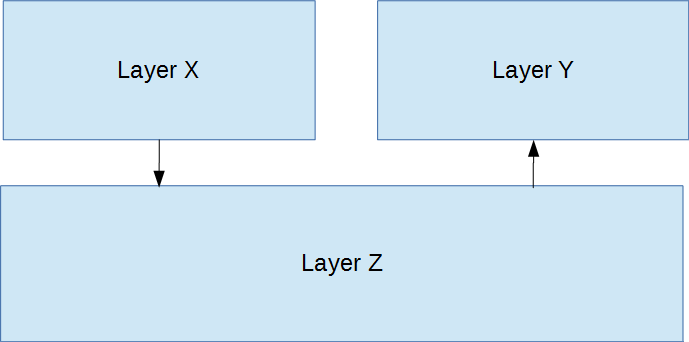
\includegraphics[width=0.60\textwidth]{images/layers}
 \caption{A simple architectural layer diagram}
\end{figure}

\subsection{Layer X Description}
Each layer should be described separately in detail. Descriptions should include the features, functions, critical interfaces and interactions of the layer. The description should clearly define the services that the layer provides. Also include any conventions that your team will use in describing the structure: naming conventions for layers, subsystems, modules, and data flows; interface specifications; how layers and subsystems are defined; etc. 

\subsection{Layer Y Description}
Each layer should be described separately in detail. Descriptions should include the features, functions, critical interfaces and interactions of the layer. The description should clearly define the services that the layer provides. Also include any conventions that your team will use in describing the structure: naming conventions for layers, subsystems, modules, and data flows; interface specifications; how layers and subsystems are defined; etc. 

\subsection{Layer Z Description}
Each layer should be described separately in detail. Descriptions should include the features, functions, critical interfaces and interactions of the layer. The description should clearly define the services that the layer provides. Also include any conventions that your team will use in describing the structure: naming conventions for layers, subsystems, modules, and data flows; interface specifications; how layers and subsystems are defined; etc. 
\section{Roles \& Responsibilities}
Who are the stakeholders of the project? Who will be the point of contact from the sponsor or customer side? Who are the team members, and what will be their areas of responsibility? Will your team maintain the product owner and scrum master for the whole project, or will that role change periodically? This section should occupy 1/2 - 1 full page.
\section{Cost Proposal}
The budget will be \$800 (can increase at the discretion of Professor Mcmurrough).  The money will come from UTA.  At this time our expectation is that the components will require a budget of \$400; this will include things like sensors and micro-controllers.  Our fabrication costs will be estimated at \$200 dollars, and the software takes the remaining budget with \$200.

\subsection{Preliminary Budget}
\begin{table}[h]
\resizebox{!}{!}{
\begin{tabular}{|l|l|}
\hline
 \textbf{Preliminary Budget} & \textbf{Allocated Budget} \\ \hline
 Components & \$400 \\ \hline
 Fabrication & \$200 \\ \hline
 Software & \$200 \\ \hline
 
\end{tabular}}
\end{table}

\subsection{Current \& Pending Support}
Currently our main funding source is from UTA.  There hasn't really been any potential funding sources because this isn't currently a sponsored project.  The current funding source is from the UTA CSE department, at a budget of \$800.
\section{Facilities \& Equipment}
The main lab space that will be utilised is the work lab provided by the senior design course at UTA in ERB 335; it will most likely be our main area of work, especially when tinkering with hardware. In terms of makerspaces, UTA provides that equipment in their library and in Nedderman Hall.  There is no guarantee that we will be using the makerspace equipment, but it's something that we can resort to in order to solve problems or implement features. For testing grounds, UTA has designated safe fly zones; places with high traffic like dorms or the library mall are absolutely prohibited, so we are relegated to the following places:  
\begin{itemize}
    \item The UTA Ballpark (as long as there's no event going on)
    \item The Maverick's Activity Center indoor soccer court (with an appointment)
    \item Inside College Park Center (with an appointment and 107 or greater pilot certification)
    \item The UTA Research Institute (with an appointment)
\end{itemize}
In terms of equipment:
\begin{itemize}
    \item drone (no purchase, UTA provided)
    \item Raspberry Pi (no purchase, internally provided)
    \item TM4C123GH6PMI Microcontroller (no purchase, internally provided)
    \item Respeaker 6-mic Array with ADC (purchase)
    \item PiJuice rechargeable battery (purchase)
\end{itemize}
\section{Assumptions}
An assumption is a belief of what you assume to be true in the future. You make assumptions based on your knowledge, experience or the information available on hand. These are anticipated events or circumstances that are expected to occur during your project's life cycle.

Assumptions are supposed to be true but do not necessarily end up being true. Sometimes they may turn out to be false, which can affect your project significantly. They add risks to the project because they may or may not be true. For example, if you are working on an outdoor unmanned vehicle, are you assuming that testing space will be available when needed? Are you relying on an external team or contractor to provide a certain subsystem on time? If you are working at a customer facility or deploying on their computing infrastructure, are you assuming you will be granted physical access or network credentials?

This section should contain a list of at least 5 of the most critical assumptions related to your project. For example:

The following list contains critical assumptions related to the implementation and testing of the project.

\begin{itemize}
  \item A suitable outdoor testing location will be available by the 3rd sprint cycle
  \item The X sensing system developed by Sensor Consulting Company will be delivered according to specifications by the 4th sprint cycle
  \item Access to the customer installation site will be provided by the 5th sprint cycle
  \item The customer will provide ample power and network connectivity at the installation site
  \item The installation site network infrastructure will allow TCP network traffic on port 8080
\end{itemize}
\section{Constraints}
The following list contains key constraints related to the implementation and testing of the project.

\begin{itemize}
  \item Final prototype demonstration must be completed by May, 2023
  \item Limited types and number of sensors can be integrated in the Raspberry Pi/embedded system
  \item Team members will not be available to work full time on the project since they are currently full time students.
  \item Total development costs must not exceed \$800
  \item Information relay from sensor system to web app through university WiFi would need approval.
  \item All data obtained from customer site must be reviewed and approved for release by the Information Security Office prior to being copied to any internet connected storage medium.
\end{itemize}


\section{Risks}
This section should contain a list of at least 5 of the most critical risks related to your project. Additionally, the probability of occurrence, size of loss, and risk exposure should be listed. For size of loss, express units as the number of days by which the project schedule would be delayed. For risk exposure, multiply the size of loss by the probability of occurrence to obtain the exposure in days. For example:

The following high-level risk census contains identified project risks with the highest exposure. Mitigation strategies will be discussed in future planning sessions.

\begin{table}[h]
\resizebox{\textwidth}{!}{
\begin{tabular}{|l|l|l|l|}
\hline
 \textbf{Risk description} & \textbf{Probability} & \textbf{Loss (days)} & \textbf{Exposure (days)} \\ \hline
 Availability of X sensor module due to contractor delay  & 0.50 & 20 & 10 \\ \hline
 Outdoor testing grounds are not available  & 0.20 & 14 & 2.8 \\ \hline
 Internet access not available at installation site  & 0.30 & 9 & 2.7 \\ \hline
 Delays in shipping from overseas vendors  & 0.10 & 20 & 2.0 \\ \hline
 Certification delays at compliance testing facility & 0.15 & 10 & 1.5 \\ \hline
\end{tabular}}
\caption{Overview of highest exposure project risks} 
\end{table}
\section{Documentation \& Reporting}
%%% In this section, you will describe all of the various artifacts that you will generate and maintain during the project life cycle. Describe the purpose of each item below, how the content will be generated, where it will be stored, how often it will be updated, etc. Replace the default text for each section with your own description. Reword this paragraph as appropriate.

\subsection{Major Documentation Deliverables}
The major deliverables are this project charter, system requirements specification, architectural design specification, and detailed design specification. These are the main documents that will be turned in during the first half of the project. Each of these document will be prepared with the co-operation of the whole team and stored in team's github as we move forward with the project. These documents will also be updated as needed during the course of the project. 

\subsubsection{Project Charter}
This document will be maintained as a team and updated during each sprint if any requirement is edited, added or removed. The initial version will be delivered on October 3rd, 2022 and the final version will be delivered along with the complete project on May of 2023.

\subsubsection{System Requirements Specification}
This document will be maintained as a team and updated as needed. The requirements will not be edited as much as other documents, but it will be updated if the team decides to add or remove some parts. The initial version will be delivered towards the end of October 2022 and the final version will be delivered along with the complete project on May of 2023.

\subsubsection{Architectural Design Specification}
This document will be maintained as a team and updated frequently during the first half of the project. In the second half as we progress in the project and we have a solid structure for the project, it will be updated few times. The initial version will be delivered on November of 2022 and the final version will be delivered along with the complete project on May of 2023.

\subsubsection{Detailed Design Specification}
This document will be maintained as a team and updated frequently during the initial stages. However, it will not be updated much after the completion of the design of the project. If a major change happens in the project, it will be updated accordingly. The initial version will be delivered on October 3rd, 2022 and the final version will be delivered along with the complete project on May of 2023.

\subsection{Recurring Sprint Items}
\subsubsection{Product Backlog}
The items will be added after the discussion with the whole team after splitting up tasks so that no item on the backlog is too big. These items will be prioritized according to the need for the software. The decisions will be based on the majority vote. The software to maintain and share the product backlog with team members and stakeholders will be Jira.

\subsubsection{Sprint Planning}
Each sprint will be planned before the beginning of the sprint. The backlog can be updated during the sprint. In Senior Design 1, there will be 4 sprints. In Senior Design 2, there will also be 4 sprints.

\subsubsection{Sprint Goal}
The Sprint goal is decided by the group together with some feedback from the sponsor and customers of the project. 

\subsubsection{Sprint Backlog}
The team together will decide the backlog items and they will be kept in the Jira Board by the scrum master. The backlog will be maintained by the whole team as they progress in their allocated tasks with options like in-progress, done, etc.

\subsubsection{Task Breakdown}
Individual task will be assigned by group discussion and the preference of each member. If there is a conflict, then the group leader for the sprint will decide how the conflicted task will be divided. Time spent on tasks will be documented using man hour.

\subsubsection{Sprint Burn Down Charts}
The scrum master will be responsible for generating the burn down charts for each sprint. The Jira Board has a feature to keep track of time spent on each task and Jira Board will create a burn down chart accordingly.

\begin{figure}[h!]
    \centering
    
\includegraphics[width=0.5\textwidth]{images/test_image}
    \caption{Example sprint burn down chart}
\end{figure}

\subsubsection{Sprint Retrospective}
How will the sprint retrospective be handled as a team? When will this discussion happen after each sprint? What will be documented as a group and as individuals, and when will it be due?
The Sprint retrospective will be handled after the day of completion of each sprint. As a group, problems faced, lessons learned, ways to improve communication and the allocation of task will be documented. As individuals, lessons learned and peer reviews will be documented. These are due according to the schedule provided by the professor.

\subsubsection{Individual Status Reports}
In the progress discussion meeting, each member will discuss the progress made by them and the problems they faced. The key items that will be included in the report will be which items they have worked on, problems they faced, if they need any assistance, etc.

\subsubsection{Engineering Notebooks}
The engineering notebook will be updated after a change is brought up in the project. At a minimum, it will be updated bi-weekly which is the length of each sprint. There will be no minimum amount of pages. Team members will be each others' witness and will keep each other accountable.

\subsection{Closeout Materials}
\subsubsection{System Prototype}
What will be included in the final system prototype? How and when will this be demonstrated? Will there be a Prototype Acceptance Test (PAT) with your customer? Will anything be demonstrated off-site? If so, will there be a Field Acceptance Test (FAT)?
The system prototype will include....................

\subsubsection{Project Poster}
Currently, this has not been discussed and will be done in the later part of the project.

\subsubsection{Web Page}
What will be included on the project web page? Will it be accessible to the public? When will this be delivered? Will it be updated throughout the project, or just provided at closeout (at a minimum, you need to provide a simple web page at the end).
The project web page will include 

\subsubsection{Demo Video}
What will be shown in the demo video(s)? Will you include a B-reel footage for future video cuts? Approximately how long will the video(s) be, and what topics will be covered?

\subsubsection{Source Code}
How will your source code be maintained? What version control system will you adopt? Will source code be provided to the customer, or binaries only? If source code is provided, how will it be turned over to the customer? Will the project be open sourced to the general public? If so, what are the license terms (GNU, GPL, MIT, etc.). Where will the license terms be listed (in each source file, in a single readme file, etc.).

\subsubsection{Source Code Documentation}
What documentation standards will be employed? Will you use tools to generate the documentation (Doxygen, Javadocs, etc.). In what format will the final documentation be provided (PDF, browsable HTML, etc.)?

\subsubsection{Hardware Schematics}
Will you be creating printed circuit boards (PCBs) or wiring components together? If so, list each applicable schematic and what sort of data it will contain (PCB layout, wiring diagram, etc.). If your project is purely software, omit this section.

\subsubsection{CAD files}
Will the project involve any mechanical design, such as 3D printed or laser-cut parts? If so, what software will you use to generate the files and what file formats will you provide in your closeout materials (STL, STEP, OBJ, etc.). If your project is purely software, omit this section.

\subsubsection{Installation Scripts}
How will the customer deploy software to new installations? Will you provide installation scripts, install programs, or any other tools to improve the process? Will there be multiple scripts provided (perhaps separate scripts for the graphical front end and back end server software)? 

\subsubsection{User Manual}
Will you customer need a printed or digital user manual? Will they need a setup video? Decide now what will be provided and discuss.

\newpage

%%% References
\bibliographystyle{plain}
\bibliographystyle{reference/IEEEtran_custom}
\bibliography{reference/refs}{}

\end{document}
